\chapter[Metodologia]{Metodologia}


% RASCUNHO (PROJETO DO CAPÍTULO)
% METODOLOGIA
% 3.1 MATERIAIS
%     -- (PPI[HPRD, MINT INTACT], EXP[KATO], SEMENTES[LINK+APENDICE])
% ==> REVISAR QUAL A IDEIA DO TCC, OU SEJA, O QUE VOCÊ DESEJA DESCOBRIR?
% ==> SE O METODO É ROBUSTO, OU SEJA, O QUANTO OS RESULTADOS VARIAM APOS ALTERAR A ENTRADA (SEMENTES) 
% ==> COMO REALIZOU OS EXPERIMENTOS?c

% 3.2 Métodos utilizado para análise de robustez
%       -- MÉTODO DE REMOÇÃO DE UM ÚNICO GENE (METODO SIMILAR AO LEAVE ONE OUT)
%       -- MÉTODO DE REMOÇÃO DE VÁRIOS (SIMILAR AO CROSS VALIDATION) ==> 

% 3.2 VALIDAÇÃO (RODOU ALGUM EXPERIMENTO SEM REMOVER NINGUEM E COMPAROU COM OS RESULTADOS ORIGINAIS?)
% 



%
Para análise de robustez do Método NERI foram utilizados conceitos de validação baseados na alteração dos genes sementes. Para que seja feita a análise foram utilizados os resultados de priorização gênica gerada pela ferramenta. De forma a ser possível verificar e mapear os impactos causados devido a remoção ou falta de genes sementes no experimento. 

\section{Materiais}

%
Este trabalho utilizou a base de dados \textsl{\textbf{KATO}} que consiste em expressões gênicas de pessoas portadoras da doença \textsl{Esquizofrenia}.
Estes dados podem ser encontrados no \textsl{Stanley Neuropathology Consortium Integrative Database (SNCID)}\footnote{SNCID: (http://sncid.stanleyresearch.org)}.
Esta base de dados em específico, foi selecionada devido ao fato de ter sido utilizada na tese de doutorado \ref{Simoes2015} no qual este trabalho se baseia e se referencia.
Assim sendo, os dados obtidos podem ser comparados com os encontrados e apresentados pelo autor, evitando o enviesamento do resultado por diferença de experimentação.

%
O Método NERI também recebe dados de rede de integração proteína proteína \textsl{(Protein Protein Interaction – PPI)}, onde os mesmos também foram mantidos os originais utilizados pelo autor, sendo formada pelas pelas bases de dados \textsl{\textbf{HPRD}}\footnote{HPRD: (http://www.hprd.org/)} (\textsl{Human Protein Reference Database}), \textsl{\textbf{MINT}}\footnote{MINT: (http://mint.bio.uniroma2.it/)} (\textsl{Molecular INTeraction database}) e \textsl{\textbf{IntAct}}\footnote{IntAct: (http://www.ebi.ac.uk/intact/)} (\textsl{IntAct molecular interaction database}).
%
Como entrada do sistema, também são definidos os \textsl{\textbf{Genes Sementes}}. Estes no qual, são os genes onde há certeza da sua relação com a doença analisada em questão, a base de dados original pode ser encontrada no apêndice~\ref{table_original_seeds}.

\section{Estratégia utilizada para análise de robustez}

%
Neste trabalho, foi escolhida a remoção de alguns genes sementes como parâmetro de análise de robustez do Método NERI. Onde o objetivo é identificar o impacto gerado na rede de integração gênica e no resultado final (lista de priorização gênica). Desta forma, podendo calcular a dependência e sensibilidade do método em relação a qualidade e quantidade de genes sementes.
%
Os métodos escolhidos para análise de robustez baseiam-se nos métodos de avaliação de classificadores \textit{Leave-one-out Cross-Validation} e \textit{Repeated K-Fold Cross-Validation}.


\subsection{Remoção de um único gene semente}

Foi utilizado um modelo baseado no método validação \textsl{Leave-one-out Cross-Validation}, onde consiste na remoção de um gene semente por vez. Desta forma, formando um \textsl{\textbf{conjunto diferente}} para cada \textsl{\textbf{gene semente}} removido, garantindo que sempre haja a mesma quantidade de genes em cada conjunto e que todos \textsl{\textbf{genes sementes}} tenham ficado de fora pelo menos uma vez. Assim sendo, o número final de conjuntos formados será a quantidade total de genes sementes.

%
Com este método, é possível descobrir se a falta de um único gene semente é responsável por alterar significantemente a priorização gênica gerada pelo Método NERI. Desta forma, podendo analisar se o método em questão é sensível a retiradas de \textsl{\textbf{genes sementes}}. 
O método de \textsl{\textbf{remoção de um único gene}} também permite a análise de importância relativa dos \textsl{\textbf{genes sementes}}, onde aquele que causar maior impacto no resultado final indica uma importância relativa maior em relação aos outros. 

%
Também é possível observar se existe relação entre as medidas de centralidade do gene representado na rede (neste trabalho, utilizaremos somente o grau do nó), com o impacto causado. Este é um ponto importante a ser analisado, pelo fato de poder estimar a importância relativa de um gene semente, observando o seu grau na rede de integração. Esta é uma medida que poderá impactar no resultado da priorização gênica resultante do Método NERI, por isso a importância da análise.


%Porém há outra análise importante que deve ser feita mas o Leave One Out não é capaz de prover, é se a quantidade de nós removidos influenciam diretamente no resultado. Para observar este aspecto, utilizamos o método Cross Validation, no qual, suas características se moldam mais a esta ótica de estudo.


\subsection{Remoção de vários genes sementes}

Foi utilizado um modelo baseado no \textsl{Repeated K-Fold Cross-Validation}, que consiste na remoção de mais de um gene semente por experimento.
%
Este método foi adotado pela sua característica principal, organização de conjuntos de genes sementes com tamanhos variados.
Com esta característica chave, buscou-se estudar o impacto dos resultados de priorização do método quando há a remoção de vários genes sementes do conjunto original.

% 
Com isso, é possível a observação dos conjuntos no qual foram removidos genes que causaram alto impacto em sua remoção na etapa anterior. Estes conjuntos informarão se o impacto na remoção de um único gene é acumulativo, ou seja, se houver a remoção de mais de um gene semente com alto impacto em sua remoção, se o resultado do experimento em questão será proporcional ao estudo da análise anterior.

\section{Definição dos genes sementes utilizados}

%
Em seu trabalho, os autores \cite{Simoes2015} utilizaram um conjunto de 38 genes sementes obtidos de um estudo de associação de esquizofrenia, apresentados na Tabela~\ref{table_original_seeds} presente no Apêndice \ref{appendice_tables}.
%
%A Tabela~\ref{table_original_seeds} apresentada no capítulo 4 apresenta estes \textsl{\textbf{38}} genes.
%
No entanto, como o Método NERI utiliza a rede \textsl{PPI}, durante a integração dos genes sementes, somente \textsl{\textbf{30}} genes foram integrados a rede. Estes nos quais foram utilizados neste trabalho, em vista que os genes sementes que não integraram não afetam o resultado final, ficando de fora dos conjuntos de genes sementes gerados para validação.

\subsection{Aplicação do método similar ao  \textsl{Leave-one-out Cross-Validation}}

Para a validação utilizando o Método similar ao \textsl{Leave-one-out Cross-Validation}, em que neste trabalho chamaremos de \textsl{\textbf{Método de remoção de apenas um gene}}, a preparação do experimento consistiu em gerar conjuntos de genes sementes para o Método NERI de forma que cada conjunto tenha um gene a menos em relação ao experimento original. Foi criado para cada gene semente, um conjunto sem o mesmo, onde exista um conjunto para cada gene removido, ou seja, em uma amostra de \textsl{\textbf{30}} genes sementes, temos \textsl{\textbf{30}} experimentos possíveis.

A aplicação direta no sistema consiste em cada execução independente do programa. Onde cada experimento seja um conjunto formado da remoção de um gene semente da amostra original. Deve existir um experimento para cada gene semente removido, garantindo que cada gene semente tenha ficado de fora uma vez em relação a todos os experimentos.

%<Para preparação destas entradas, foi desenvolvido um script em Python 3.X para automatização do processo e para evitar falha humana.>

%<Script Python GERA LOO>

%
Para ilustração do experimento, segue o exemplo: Suponha que exista um conjunto de \{\textsl{\textbf{5}} genes sementes \{\textsl{\textbf{1,2,3,4,5}}\}, suponha que deseja-se gerar todos os possíveis conjuntos de genes sementes utilizando o método de \textsl{\textbf{remoção de apenas um gene}}.
A Tabela~\ref{table_loo_example} representa os conjuntos resultantes, onde \textsl{\textbf{$S_i$}} é o i-ésimo subconjunto gerado.

%
% ======================= TABELA LOO EXEMPLO ==================
\begin{table}[]
\centering
\caption{Tabela representativa. Experimentos resultantes do método de remoção apenas um gene}
\label{table_loo_example}
\begin{tabular}{@{}lll@{}}
\toprule
\textbf{\textsl{Conjunto}} & \textbf{\textsl{Elementos}} \\ \midrule
\textsl{\textbf{$S_1$}} & 2,3,4,5 \\
\textsl{\textbf{$S_2$}} & 1,3,4,5 \\
\textsl{\textbf{$S_3$}} & 1,2,4,5 \\
\textsl{\textbf{$S_4$}} & 1,2,3,4 \\ \bottomrule
\end{tabular}
\flushleft{
Subconjuntos gerados pelo método de remoção de apenas um gene no conjunto de genes sementes \textbf{\{\textsl{1,2,3,4,5}\}}, sendo $S_i$ o i-ésimo subconjunto gerado.

Fonte: Tabela gerada pelo autor.}
\end{table}
%
% ======================= FIM TABELA LOO EXEMPLO ===============

\subsection{Aplicação do método similar ao \textsl{Repeated K-Fold Cross-Validation}}

Para a validação utilizando o Método similar ao \textsl{Repeated K-Fold Cross-Validation}, em que neste trabalho chamaremos de \textsl{\textbf{Método de remoção de mais de um gene}},
%
inicialmente, foi definido o tamanho dos grupos de genes sementes de entrada a serem removidos para cada bateria de execuções.
Levando em consideração a quantidade de genes de entrada total do experimento, \textsl{\textbf{30}} após a integração com a rede \textsl{PPI}, definiu-se que as remoções seriam feitas em relação a porcentagem da amostra original, sendo as porcentagens definidas \textbf{\textsl{10\%}} (3 genes), \textsl{\textbf{20\%}} (6 genes),\textsl{\textbf{30\%}} (9 genes) e \textsl{\textbf{40\%}} (12 genes), conforme pode ser observado na tabela \ref{table_gene_execucao}. Também representada na tabela, determinou-se a quantidade de agrupamentos de dados de entrada para cada porcentagem de remoção.

\begin{table}[]
\centering
\caption{Tabela representativa. Porcentagem de genes sementes removidos em relação aos \textsl{\textbf{30}} genes sementes originais e suas respectivas porcentagens}
\label{table_gene_execucao}
\begin{tabular}{@{}ccc@{}}
\toprule
\textbf{\textsl{Quantidade de}} & \textbf{\textsl{Porcentagem de}} & \textbf{Quantidade de} \\ 
\textbf{\textsl{genes removidos}} & \textbf{\textsl{remoção}} & \textbf{Experimentos} \\ \midrule
3 & 10\% & 50 \\
6 & 20\% & 50 \\
9 & 30\% & 50 \\
12& 40\% & 50 \\ \bottomrule
\end{tabular}
\flushleft{Fonte: Tabela gerada pelo autor.}
\end{table}

Para uma maior diversidade dos resultados, o método foi implementado de forma que cada grupo fosse diferente do outro.
%
Isso visa garantir que o conjunto de genes removidos não se repita dentro de cada etapa, para evitar executar o mesmo experimento mais de uma vez.
Assim, inicialmente são geradas todas as \textsl{\textbf{50}} combinações dos genes a serem removidos e em seguida são realizados os \textsl{\textbf{50}} experimentos.
%
O script que gera todas as combinações de N genes em M experimentos foi desenvolvido em \textsl{\textbf{Python 3.x}} e pode ser encontrado no Anexo~\ref{CVV_script}.


A Figura~\ref{cvv_explanation} ilustra o o processo de criação dos experimentos.
%
Para uma melhor compreensão, segue o exemplo abaixo.
Suponha que exista um conjunto de com 10 genes sementes: \{\textsl{\textbf{0,1,2,3,4,5,6,7,8,9}}\}, e suponha que deseja-se gerar 5 conjuntos de genes sementes com um percentual de remoção em \textsl{\textbf{20\%}}.
%
Assim, dado \textsl{\textbf{20\%}} de \textsl{\textbf{10}} elementos, temos \textsl{\textbf{fator de remoção = 2}} elementos.
Seja $S_i$ o i-ésimo subconjunto gerado cujo o respectivo conjunto de genes removidos é $R_i$
Portanto, um exemplo dos 5 subconjuntos está abaixo:

\begin{lstlisting}
    S1 = {0,1,2,3,4,5,6,7}
    S2 = {0,1,2,3,4,5,6,8}
    S3 = {0,1,2,3,4,5,6,9}
    S4 = {1,2,3,4,5,6,7,8}
    S5 = {2,3,4,5,6,7,8,9}
\end{lstlisting}

Sendo $R_i$ os conjuntos dos elementos removidos:

\begin{lstlisting}
    R1 = {8,9}
    R2 = {7,9}
    R3 = {7,8}
    R4 = {0,9}
    R5 = {0,1} 
\end{lstlisting}

%Imagem desenhada no caderninho
%Imagem
\begin{figure}[ht!]
\centering
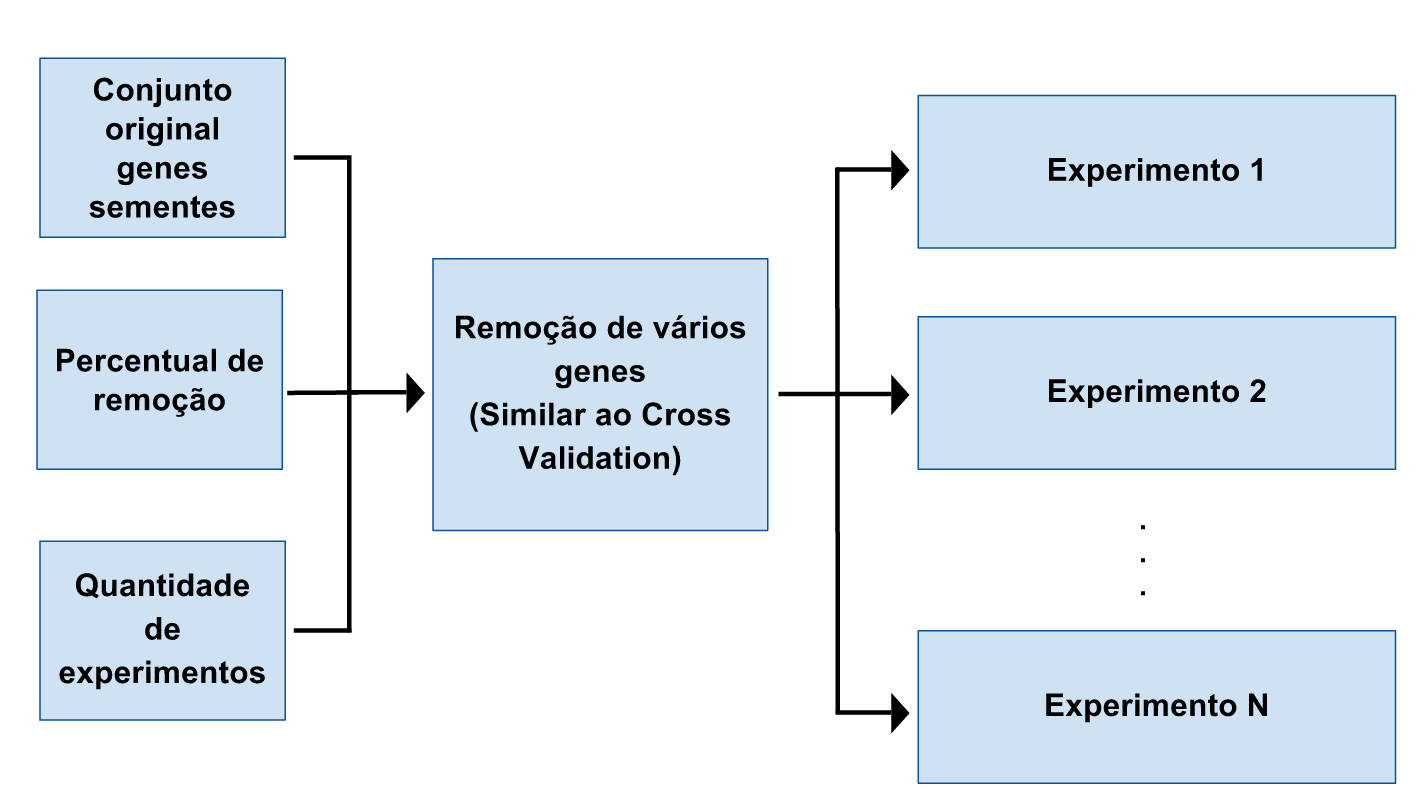
\includegraphics[width=\textwidth]{Images/flows/cvv_explanation.png}
\caption {Fluxograma de funcionamento da remoção de vários genes sementes.
\label{cvv_explanation}}
\flushleft{Fonte: Produzido pelos autores.}
\end{figure}
%


Após os agrupamentos de dados de entrada serem preparados, o programa principal é executado individualmente para cada agrupamento. Totalizam-se 200 execuções individuais do programa que implementa o Método NERI.

\section{Execução dos experimentos}

%
% DETALHAR MAIS OS EXPERIMENTOS
% 
Nesta etapa, os experimentos encontram-se preparados para execução direta no programa principal que implementa o Método NERI.
%
Primeiramente, realizamos experimentos com a remoção de um único gene, para cada um dos \textsl{\textbf{30}} genes, o que totalizou \textsl{\textbf{30}} experimentos.
%
Em seguida, realizamos \textsl{\textbf{50}} experimentos para cada percentual de remoção (\textsl{\textbf{10\%}}, \textsl{\textbf{20\%}}, \textsl{\textbf{30\%}}, \textsl{\textbf{40\%}}), totalizando \textsl{\textbf{200}} experimentos nesta etapa.

%
Devido ao fato de o programa realizar cálculos demorados, houve a necessidade de automatização do processo de execução, onde foi desenvolvido um \textsl{Script} em \textsl{Shell} (linha de comando Linux), para efetuação do trabalho, podendo ser encontrado no apêndice~\ref{shell_run_all}.
Além disso, houve uma padronização nos diretórios utilizados pelo método NERI, a fim de identificar os experimentos realizados, conforme pode ser observado na Figura~\ref{tree_files} presente no Apêndice~\ref{appendice_ambient}.
% DIRETORIO
% INPUT | DADOS DE ENTRADO DO USUARIO X Y E Z
% OUTPUT | RESULTADOS COM IDENTIFICADOR IGUAL AO DIRETORIO DE ENTRADA(+-)
% ...

%
Juntamente com as alterações estruturais, também foi desenvolvida uma \textsl{\textbf{interface gráfica}} e uma interface em \textsl{\textbf{linha de comando}} (\textsl{CLI}), para facilitar a utilização por pessoas que não possuem familiaridade com este modelo de execução de programas.
Essa interface está em fase de finalização, faltando a documentação e alguns ajustes, e assim que estiver finalizada será disponibilizada livremente na web.

\section{Validação}
%
Para garantir que não houvesse erro nos resultados devido a algum erro proveniente a configuração do ambiente de testes ou em relação as bases de dados utilizadas, foi executado o experimento original \textsl{\textbf{KATO}}. O resultado apresentado foi praticamente o mesmo, apresentando pequenos erros nas casas decimais \textsl{\textbf{$10^{-20}$}} provenientes por algum erro de arredondamento causado pela arquitetura do computador em questão, também pode ser levado em consideração atualizações das bibliotecas utilizadas pelo \textsl{\textbf{programa NERI}}. Estes erros foram muito baixos e não influenciaram no resultado final gerado pelo programa. %O resultado comparativo dos experimentos bases podem ser observados na Tabela~\ref{}.

\section{Metologia de análise dos resultados}

% ==> REESCREVER
Após as execuções dos experimentos definidos, tivemos que definir as métricas para análise dos resultados.
O Método NERI realiza uma priorização gênica, produzindo como saída dois escores de ranqueamento ($\Delta'$ e $X$) para cada gene.
Assim, são produzidas duas listas (uma lista para o escore $X$ e outra para o escore $\Delta'$), cada uma contendo os genes que participaram dos caminhos mínimos selecionados. 

Assim, após a remoção dos genes sementes, realizamos uma comparação de ambas as listas resultantes com a lista original.
Essa comparação foi realizada tomando-se os primeiros genes N genes obtidos na lista do experimento e comparando-os com a respectiva lista original.
O valor N dos primeiros genes da lista foi variado em \{\textsl{\textbf{10}}, \textsl{\textbf{20}}, \textsl{\textbf{50}}, \textsl{\textbf{100}}\}, e para cada um foi feita a comparação da interseção.


% CHECAR AS PALAVRAS CORRELAÇÕES USADAS INDEVIDAMENTE
% remover o devido 
% ====== VERIFICAR SE VOU DEIXAR OU NAO O SPEARMAN
Para comparar duas listas ordenadas, geralmente utiliza-se a \textsl{\textbf{Correlação de Spearman}}.
Em nossos testes, inicialmente utilizamos essa correlação para compararmos as listas geradas pelos \textsl{\textbf{experimentos deste trabalho}} com a lista gerada pelo \textsl{\textbf{experimento original}}.
%
Observamos que, apesar de haver uma interseção razoável dos primeiros genes encontrados em ambas as listas,  a comparação utilizando a \textsl{\textbf{Correlação de Spearman}} apresentou valores próximos de zero, visto que esta medida penaliza listas que não estiverem na mesma ordem.
%
Assim, a \textsl{\textbf{Correlação de Spearman}} não mostrou-se um bom fator de comparação, pelo fato de a ordem dos genes em um grupo não ser a preocupação principal, mas sim se os genes foram escolhidos para estarem naquele agrupamento.


Muitas vez um biólogo pode estar mais preocupado com a \textsl{\textbf{replicabilidade}} de um experimento do que com a ordem dos genes priorizados.
Isto é, se os genes recuperados em um método são, em sua maioria, os mesmos recuperados em outro método.
Desta forma, algumas vezes pode ser mais importante comparar a interseção das listas do que a ordem das mesmas.
Assim, para a análise dos resultados, comparamos as interseções dos \textsl{\textbf{N}} primeiros genes de cada lista, variando \textsl{\textbf{N}} em \textsl{\textbf{\{10,20,50,100,200\}}}.


%====== FIM SPEARMAN

Foi utilizada a \textsl{\textbf{comparação por interseção}}, onde consiste em verificar a porcentagem de elementos presentes nas duas listas, de forma que o resultado indique o quão parecido os conjuntos são em relação a presença dos elementos iguais.
Sendo definido matematicamente por: 
$I = {{A \cup B} \over |A|}$

Este modelo de comparação beneficia as listas que possuírem mais elementos iguais, porém não penaliza as listas seccionadas que tiveram a ordem relativa dos elementos alterada. Este é um fator importante, pois o objetivo da análise é verificar a \textsl{\textbf{replicabilidade}} do experimento em condições diferenciadas, logo ligeiras variações de posicionamento dos elementos não são problemáticas, desde que os elementos das listas comparadas sejam iguais ou o possuírem uma grande interseçã com o resultado otiginal.


% ======================== EXEMPLOS TEX ========================
%Exemplo codigo no TEX
%\begin{lstlisting}[caption={Código fonte do método getBlockStatic da classe %Tools.},label=getBlockStatic,language=Java]
%public static List<Rect> getBlockStatic(Bitmap bmp, int nr, int nrTotal) {
%    Mat mat = bitmapToMat(bmp);
%    Size size = mat.size();
%    List<Rect> list = new ArrayList<>();
%    int left, top, rigth, bottom;
%    for (int i = 0; i < nrTotal; i++) {
%        top = 0;
%        if (i == 0) {
%            left = 1;
%        } else {
%            left = 1 + (mat.cols() / nrTotal * i);
%        }
%        bottom = mat.rows();
%        rigth = left + (mat.cols() / nrTotal);
%        list.add(new Rect(left, top, rigth - 1, bottom - 1));
%    }
%    List<Rect> result = new ArrayList<>();
%    for (int j = nr - 1; j < 4; j++) {
%        result.add(list.get(j));
%    }
%    list = null;
%    return result;
%}
%\end{lstlisting}